\section{Опыт работы}

Основным направлением деятельности Asure в сфере социального обеспечения является пенсионное страхование. В рамках продолжающегося исследования мы перенесли специфические аспекты немецкой пенсионной системы в блокчейн Ethereum. Основываясь как на нашем практическом опыте, так и на опыте, накопленном за годы работы в области страхования, мы разработали теоретическую основу функционирования децентрализованной пенсионной системы, а также практическую реализацию такой системы. 

\subsection{Исследования технологии блокчейн и автоматизации}

Технический директор Asure, Фабиан Рец (Fabian Raetz), в 2013 году провел исследовательский проект в Университете прикладной науки и искусства в Дортмунде, где проанализировал новые технологии блокчейна и их возможное приминение. \cite{fraetz}
\newline

В 2014 году небольшая команда во главе с Полом Мизелем (Paul Mizel) и Фабианом Райцем (Fabian Raetz) разработала собственную валюту, основанную на блокчейне в качестве доказательства концепции и проверила различные виды проблем блокчейна и экономические системы (монета NRJ). \cite{nrjcoin}
\newline

В конце 2015 года Paul Mizel создал команду в Киеве для инновационных проектов на основе ИИ «Insure Chat», «Insure Assistant» и «Insure Advisor». В результате были созданы полностью автоматизированные чат-боты для поддержки, управления заявками и других задач с уникальным механизмом обучения и подключением к социальным платформам, таким как Facebook, Telegram, Skype и другие.\newline
Технический стек: IBM Watson, Microsoft Bot Framework, MS Luis, .NET.
\newline
Используемые алгоритмы: интеллектуальный анализ текста, регрессионный анализ, SVM, нейронные сети.

\subsection{Немецкая пенсионная система}
Чтобы продемонстрировать потенциал социального обеспечения, основанного на блокчейне, Asure создал прототип, основанный на модели немецкой государственной пенсионной системы с выплатой пенсии по факту.
\newline\newline

Asure dApp станет эталонной реализацией для dApps, использующих блокчейн и платформу Asure.
\newline\newline
Это предоставит
\begin{itemize}
\item техническое технико-экономическое обоснование пенсионной системы Германии, внедренной на блокчейне Ethereum и протоколе / платформе Asure.
\item полная реализация кошелька.
\item обзор и управление вашими страховыми полисами.
\item страховой магазин, чтобы найти и купить страховые полисы.
\end{itemize}

Пожалуйста, попробуйте Asure dApp, который в настоящее время работает на тестовой сети Ethereum Rinkiby: https://dapp.asure.io

\subsection{Децентрализованная пенсионная система}

Чтобы продемонстрировать, что блокчейн может решать проблемы в глобальном масштабе, Asure также разработала прототип глобальной пенсионной системы, которая полностью децентрализована и следовательно, не принадлежит ни правительству, ни какой-либо страховой компании.

Это эксперимент в альфа-фазе, призванный показать, как можно улучшить системы социального обеспечения в будущем с помощью технологии блокчейн.

Идея состоит в том, чтобы внедрить пенсионную систему с оплатой по факту на блокчейне Ethereum. Участники платят свои взносы в ETH и получают токены ERC20 взамен. Никакие вклады не вкладываются в рынок капитала и, следовательно, проценты не начисляются. Вместо этого, оплаченные ETH используются непосредственно для выплаты невыплаченных пенсионных требований. Сколько пенсии будет выплачиваться, зависит от того, сколько пенсионных токенов имеет пенсионер, то есть сколько взносов он внес в систему.

Как правило, системы pay-as-you-go работают только потому, что штаты вводят обязательные системы социального обеспечения и таким образом, могут гарантировать стабильное количество участников и выплаты взносов. В децентрализованной пенсионной системе никто не может быть принужден к членству. Членство в Asure создает несколько стимулов, которые должны привести к массовому принятию.

В децентрализованной пенсионной системе, как и в классической, любой кто вносит больший вклад, получает более высокую пенсию. Долгосрочные выплаты также играют роль. Чем дольше осуществляются регулярные выплаты, тем дольше будет выплачиваться пенсия.

\begin{figure}[H]
    \centering
    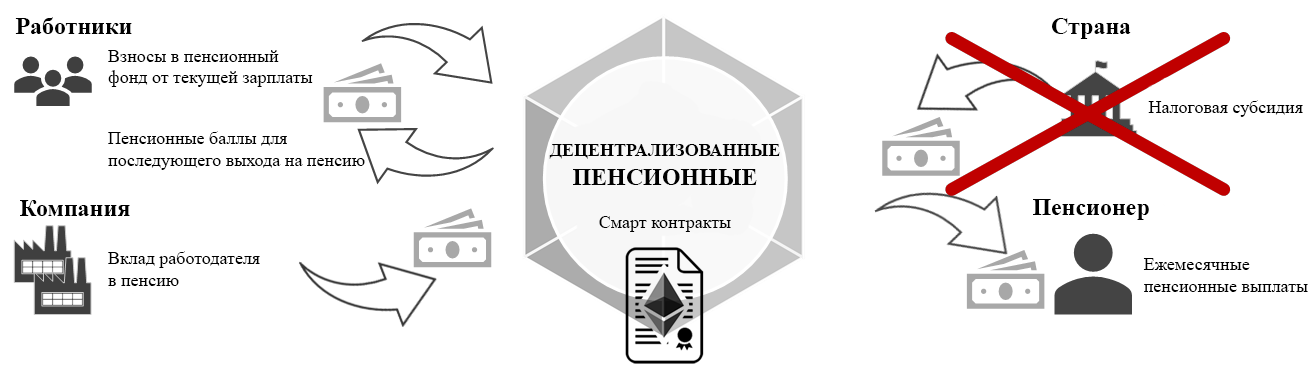
\includegraphics[width=5.0in]{img/pension.png}
    \caption{Модель PAYG}
    \label{fig:payg}
\end{figure}

В настоящее время децентрализованное пенсионное приложение Asure работает на тестовой сети Ethereum Rinkeby. Он был разработан во время ETHBerlin Hackathon и доступен по ссылке: 
\url{https://ethberlin.asure.io}

Пенсия это ставка, по которой сумма, которую я плачу, по меньшей мере так же велика, если не больше, чем выплата. Децентрализованная пенсия основана на немецкой пенсионной системе и имеет "генерационный контракт". Молодое поколение платит старшему поколению в соответствии со своими возможностями, а взамен пенсии распределяются по токенам в виде токенов пенсионных прав (PET).
\newline\newline

\subsubsection*{Модели стимулирования были разработаны в рамках проекта}
Система исключает управление возрастом, что позволяет избежать мошенничества. Время делится на периоды, где период - месяц. В течение каждого периода могут быть сделаны депозиты. Для каждого периода фиксированная целевая цена может измениться, если медиана депозитов предыдущего периода будет сильно отличаться от целевой цены. 

Если максимальное количество периодов было оплачено, также возможно максимальное количество пенсионных выплат. Предположим, что максимальное количество периодов равно 480 и равно 40 годам. Для ежемесячных выплат 40 лет, есть требование 40-летней пенсии. Если кто-то использовал систему только в течение 2 лет, заявка подана только на 1 месяц. Стимул к максимальному использованию системы вознаграждает участников с большим сроком пенсионного обеспечения.

\begin{eqnarray}
	entitlementMonths = \frac{payedMonths^2}{12 \cdot 40 years}
\end{eqnarray}

\begin{figure}[H]
    \centering
    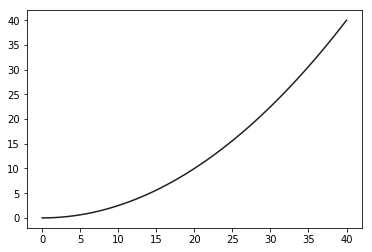
\includegraphics[width=3.0in]{img/pension_years.png}
    \caption{Децентрализованные пенсионные выплаты относительно получаемых лет}
    \label{fig:pension_years}
\end{figure}

Поскольку каждый может платить в системе разные суммы, максимальный плательщик получает максимальное двойное пенсионное право. Все те, кто платит больше, чем целевая цена периода, получат больше PET, но не более чем 2 за период. Максимально достижимые 960 PET, это позволит вам впоследствии претендовать на вдвое большее перераспределение, чем тот, кто активирует 480 PET.

\begin{eqnarray}
	DPT = \begin{cases} 1 + \frac{amount-amount_{max}}
	{targetPrice - amount_{max}} 
	* DTP_{bonus} & amount \geq targetPrice\\
	\frac{amount - amount_{min}}
	{targetPrice - amount_{min}} 
	* DTP_{bonus} & otherwise\end{cases}
\end{eqnarray}

\begin{eqnarray}
targetPrice - amount_{max} \neq 0 \quad and \quad targetPrice - amount_{min} \neq 0
\end{eqnarray}

В качестве дополнительного стимула для ранних пользователей в системе был предоставлен бонус, который имеет множитель 1.5, а время логарифмического приближения к 1.0 планируется приближать ежегодно.

\begin{eqnarray}
	DTP_{bonus} = f(year) = 1.5-0.12 * log(year)
\end{eqnarray}

\begin{figure}[H]
    \centering
    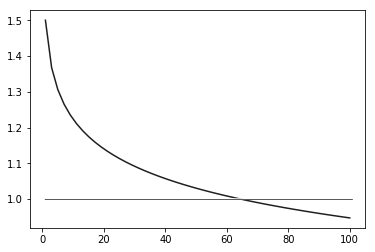
\includegraphics[width=3.0in]{img/pension_bonus.png}
    \caption{Децентрализованный пенсионный бонус по годам}
    \label{fig:pension_bonus}
\end{figure}

Если все выходят из системы, последние участники получают больше вознаграждений, поэтому мы гарантируем, что система останется прибыльной, поскольку нулевые участники системы снова будут установлены в исходное состояние.

Из-за ограничения в максимум 2 PET или с коэффициентом 1.5 первоначально 3 ПЭТ в течение периода в первые годы появляется возможность использования в системе нескольких счетов для оплаты, в которой система предотвращает передачу этих PET. 

С помощью этих стимулов и прозрачного дизайна и подхода DAO это начнется как социальный эксперимент после необходимых симуляций и корректировок параметров в сети Ethereum.

\subsubsection*{Преимущества}
Независимая крипто пенсия имеет много преимуществ, межпоколенческий контракт обеспечивает инфляционную безопасность. Он автономен и децентрализован в соответствии с идеей DAO. Там нет посредников. Конфиденциальность защищена, потому что никакие личные данные не нужны для участия в системе. Он полностью прозрачен, так как все транзакции находятся в блокчейне, а также с открытым исходным кодом.

\subsubsection*{Узнать больше}
Мы суммировали наши идеи о том, как основанная на перераспределении система взаимного пенсионного обеспечения могла бы выглядеть и поделились нашими результатами с более широким сообществом.
\newline
Depot Paper: \url{https://www.asure.network/asure.depot.en.pdf}

